%===================================================================================
% JORNADA CIENTÍFICA ESTUDIANTIL - MATCOM, UH
%===================================================================================
% Esta plantilla ha sido diseñada para ser usada en los artículos de la
% Jornada Científica Estudiantil de MatCom.
%
% Por favor, siga las instrucciones de esta plantilla y rellene en las secciones
% correspondientes.
%
% NOTA: Necesitará el archivo 'jcematcom.sty' en la misma carpeta donde esté este
%       archivo para poder utilizar esta plantilla.
%===================================================================================

%===================================================================================
% PREÁMBULO
%-----------------------------------------------------------------------------------
\documentclass[a4paper,10pt,twocolumn]{article}

%===================================================================================
% Paquetes
%-----------------------------------------------------------------------------------
\usepackage{amsmath}
\usepackage{amsfonts}
\usepackage{amssymb}
\usepackage{jcematcom}
\usepackage[utf8]{inputenc}
\usepackage{listings}
\usepackage[pdftex]{hyperref}
\usepackage{caption}
\usepackage{subcaption}
\usepackage{graphicx}
\usepackage{float}
\usepackage{xcolor}
\usepackage{tikz}
\usepackage{pgfplots}
\pgfplotsset{compat=1.18}
%-----------------------------------------------------------------------------------
% Configuración
%-----------------------------------------------------------------------------------
\hypersetup{colorlinks,%
	    citecolor=black,%
	    filecolor=black,%
	    linkcolor=black,%
	    urlcolor=blue}

% Para cambiar "Cuadro" por "Tabla"
\addto\captionsspanish{\def\tablename{Tabla}}
%===================================================================================

%===================================================================================
% Presentacion
%-----------------------------------------------------------------------------------
% Título
%-----------------------------------------------------------------------------------
\title{Modelos de Población}

%-----------------------------------------------------------------------------------
% Autores
%-----------------------------------------------------------------------------------
\author{\\
\name René Díaz González \email \href
	\\ \addr Grupo C-211 \AND
\name Gilberto Rodríguez Crespo \email \href
  \\ \addr Grupo C-211\AND
\name Gabriel Pérez Suárez \email \href
  \\ \addr Grupo C-212}


%-----------------------------------------------------------------------------------
% Tutores
%-----------------------------------------------------------------------------------
\tutors{}

%-----------------------------------------------------------------------------------
% Headings
%-----------------------------------------------------------------------------------
\jcematcomheading{\the\year}{1-\pageref{end}}{A. Uno, A. Dos}

%-----------------------------------------------------------------------------------
\ShortHeadings{Modelos Poblacionales EDO}{Autores}
%===================================================================================

%===================================================================================
% DOCUMENTO
%-----------------------------------------------------------------------------------
\begin{document}

%-----------------------------------------------------------------------------------
% NO BORRAR ESTA LINEA!
%-----------------------------------------------------------------------------------
\twocolumn[
%-----------------------------------------------------------------------------------

\maketitle

%===================================================================================
% Resumen y Abstract
%-----------------------------------------------------------------------------------
\selectlanguage{spanish} % Para producir el documento en Español

%-----------------------------------------------------------------------------------
% Resumen en Español
%-----------------------------------------------------------------------------------
\begin{abstract}
Este trabajo integra técnicas analíticas y numéricas de ecuaciones diferenciales para estudiar la dinámica de sistemas poblacionales. Se abordan tres modelos fundamentales: crecimiento no lineal con tasa proporcional a la raíz cuadrada de la población, modelo logístico con bifurcación transcrítica y sistema lineal de dos especies en interacción. Se demuestran resultados analíticos, se clasifican puntos de equilibrio, se analizan diagramas de bifurcación y se implementan métodos numéricos (Euler y Euler mejorado) con estudio de errores. Los resultados muestran la versatilidad de la modelación matemática en ecología, destacando comportamientos como crecimiento ilimitado, umbrales de supervivencia e interacciones competitivas.
\end{abstract}

%-----------------------------------------------------------------------------------
% English Abstract
%-----------------------------------------------------------------------------------
\vspace{0.5cm}

\begin{enabstract}
This work integrates analytical and numerical techniques of differential equations to study population dynamics. Three fundamental models are addressed: nonlinear growth with rate proportional to the square root of population, logistic model with transcritical bifurcation, and linear two-species interaction system. Analytical results are demonstrated, equilibrium points are classified, bifurcation diagrams are analyzed, and numerical methods (Euler and Improved Euler) are implemented with error analysis. The results show the versatility of mathematical modeling in ecology, highlighting behaviors such as unlimited growth, survival thresholds, and competitive interactions.
\end{enabstract}

%-----------------------------------------------------------------------------------
% Palabras clave
%-----------------------------------------------------------------------------------
\begin{keywords}
	Ecuaciones diferenciales, Modelos poblacionales, Bifurcación, Métodos numéricos, Estabilidad
\end{keywords}

%-----------------------------------------------------------------------------------
% Temas
%-----------------------------------------------------------------------------------
\begin{topics}
	Matemática Aplicada, Ecuaciones Diferenciales Ordinarias
\end{topics}

%-----------------------------------------------------------------------------------
% NO BORRAR ESTAS LINEAS!
%-----------------------------------------------------------------------------------
\vspace{0.8cm}
]
%-----------------------------------------------------------------------------------

%===================================================================================
% CONTENIDO PRINCIPAL - TODO EL CONTENIDO DE Proyecto EDO-Num.tex
%===================================================================================

\section{Introducción}
Este trabajo integra técnicas analíticas y geométricas de las ecuaciones diferenciales para explorar la dinámica de sistemas poblacionales. Se abordan tres escenarios fundamentales: un modelo de crecimiento no lineal, un modelo con bifurcación y un sistema de dos especies en interacción, destacando la versatilidad de la modelación matemática en ecología.

\section{Parte A: Modelo de crecimiento no lineal}

\subsection{Demostración de la ecuación diferencial}

Tenemos que $\beta$ es inversamente proporcional a $\sqrt{P}$, igual que $\delta$:
\[
\beta = \frac{b}{\sqrt{P}} \quad \text{y} \quad \delta = \frac{d}{\sqrt{P}}
\]
Y que el crecimiento poblacional es proporcional a la población:
\[
\frac{dP}{dt} = mP
\]
Dicha constante de proporcionalidad será la diferencia de las tasas de natalidad y mortalidad:
\[
m = \beta - \delta
\]
Sustituyendo beta y delta:
\[
\frac{dP}{dt} = \left(\frac{b}{\sqrt{P}} - \frac{d}{\sqrt{P}}\right)P
\]
\[
\frac{dP}{dt} = \left(\frac{b - d}{\sqrt{P}}\right)P
\]
Digamos que $k = b - d$:
\[
\frac{dP}{dt} = \frac{kP}{\sqrt{P}}
\]
Racionalizando queda:
\[
\frac{dP}{dt} = k\sqrt{P}
\]
\[
\frac{dP}{\sqrt{P}} = k\,dt
\]
Integrando ambos miembros respecto a $t$:
\[
\int\frac{dP}{\sqrt{P}} = \int k\,dt
\]
\[
2\sqrt{P} = kt + C
\]
\[
\sqrt{P} = \frac{kt + C}{2}
\]
\[
P = \left(\frac{kt + C}{2}\right)^2
\]
\[
P = \left(\frac{kt}{2}+\frac{C}{2}\right)^2
\]
\[
P(0) = \left(\frac{k\cdot0}{2}+\frac{C}{2}\right)^2
\]
\[
P(0) = \frac{C^2}{4}
\]
\[
C = 2\sqrt{P(0)}
\]
Sustituyendo $C$:
\[
P = \left(\frac{kt}{2}+\sqrt{P(0)}\right)^2
\]
Por lo que queda demostrada la ecuación diferencial.

\subsection{Valores iniciales}

Tenemos que $P(0) = 100$ y que $P(6) = 169$. Entonces $P(12) = ?$

El objetivo es hallar la $k$ que permite que la función pase por esos 3 puntos. Como $P(6) = 169$ y $P(0) = 100$:
\[
P(6) = \left(\frac{k\cdot6}{2}+\sqrt{P(0)}\right)^2 = 169
\]
\[
(3k+\sqrt{100})^2 = 169
\]
\[
(3k+10)^2 = 169
\]
\[
\sqrt{(3k+10)^2} = \sqrt{169}
\]
\[
3k+10 = 13
\]
\[
3k = 3
\]
\[
k = 1
\]
Teniendo $k$, tenemos la ecuación completamente en función de $t$. Evaluando $P(12)$:
\[
P(12) = \left(\frac{12}{2}+10\right)^2
\]
\[
P(12) = (16)^2
\]
\[
P(12) = 256
\]

Dentro de un año (12 meses) habrán 256 peces en el lago.

\subsection{Campo de isoclinas}

A continuación, se ilustra el campo de isoclinas de la ecuación diferencial $\frac{dP}{dt} = k\sqrt{P}$ donde se tomó $k = 1$.

Se muestran varias soluciones con diferentes valores de población inicial. Como la población de peces aumenta con el paso del tiempo, la tasa de natalidad es mayor que la de mortalidad, por lo que la constante $k$ debe ser positiva para que las isoclinas sean crecientes. En la figura se muestra como la función del ejercicio, con $P(0) = 100$ y $k = 1$, cumple además las otras dos condiciones, $P(6) = 169$ y $P(12) = 256$.

Para poblaciones pequeñas el crecimiento es demasiado lento, y acelerado para poblaciones medianas o grandes. Los únicos puntos críticos son $P=0$, donde la población se extingue. No hay límite superior en el modelo.

\textbf{Ver Isoclinas.ipynb}

\begin{figure}[h!]
\centering
\includegraphics[width=0.48\textwidth]{imagenes/kampliado.png}
\includegraphics[width=0.48\textwidth]{imagenes/k=1.png}
\caption{Campo de isoclinas para el modelo de crecimiento no lineal.}
\label{fig:isoclinas}
\end{figure}

\subsection{Planteamiento del Problema}

Para cada solución particular del problema, o sea, para un $k$ y $P(0)$ específicos, sabemos que:

\begin{itemize}
    \item La función solución $P(t) = (kt/2 + \sqrt{P(0)})^2$ tiene como dominio todas las $t > t_0$, ya que no tiene límite superior, por lo que para cualquier $t$ habrá una $P$ solución.
    \item $P(t)$ es inyectiva, como muestra la gráfica, garantizando la unicidad de las soluciones.
    \item $P(t)$ es continua y diferenciable, descartando cualquier inestabilidad en las soluciones.
\end{itemize}

Pero en $P = 0$ es una zona de puntos críticos, llegar aquí significa la extinción de la especie y la función se volvería constante en 0 como muestran los isoclinas ($P(t)=0$), esto descartaría la unicidad.

\textbf{En resumen:} El problema estará bien planteado siempre que ningún factor lleve a $P(t)=0$, por ejemplo: $k = 0$ o $P(0) = 0$.

\subsection{Condicionamiento del Problema}

Dado: $\frac{dP}{dt} = \sqrt{P}$, $P(0) = 100$.
Solución: $P(t) = \left(\frac{t}{2} + 10\right)^2$.

Para la solución $P(t) = \left(\frac{t}{2} + 10\right)^2$, el número de condición respecto a perturbaciones en $t$ es:
\[
\text{cond}(P, t) = \left| \frac{t \cdot P'(t)}{P(t)} \right| = \frac{2t}{t + 20}
\]

\begin{itemize}
    \item $t = 0$: $\text{cond} = 0$ (insensible)
    \item $t = 10$: $\text{cond} \approx 0.67$ (buen condicionamiento)
    \item $t \to \infty$: $\text{cond} \to 2$ (condicionamiento moderado)
\end{itemize}

\textbf{Interpretación:} Para $t$ grandes, un error del $1\%$ en $t$ produce aproximadamente un $2\%$ de error en $P(t)$.

\subsection{Métodos numéricos y errores}

En este apartado se emplean dos métodos numéricos para el mayor análisis del problema, y como otras vías de solución. Estos son el método de Euler y el método de Euler Mejorado, también conocido como método de Heun.

\textbf{Ver Euler y Euler Mejorado.ipynb}

\begin{figure}[h!]
\centering
\includegraphics[width=0.5\textwidth]{imagenes/eulermh2.png}
\caption{Comparación de métodos de Euler y Euler mejorado.}
\label{fig:euler}
\end{figure}

Del gráfico comparativo se aprecia como Euler mejorado (línea negra) logra mucha mayor precisión que el de Euler (línea azul). Euler mejorado es más preciso siendo de orden 2, calculando dos pendientes y hallando su promedio en cada iteración, si se reduce $h$ a la mitad, el error se reduce a la cuarta parte. En cambio, el método de Euler es de orden 1 y es más sencillo el cálculo de cada iteración, calculando solo una pendiente, si $h$ se reduce a la mitad, el error también se reduce a la mitad. Ambos métodos tienen complejidad temporal $O(n)$, donde $n$ es el número de iteraciones a realizar, aunque Euler mejorado realice más trabajo por iteración.

Ahora, analizaremos los errores absolutos, relativos, hacia adelante y hacia atrás de estos métodos comparados con la solución exacta.

\begin{itemize}
    \item \textbf{Error absoluto:} Se calcula como la diferencia entre la solución exacta y la aproximada: $\Delta y = \left\lvert y - \widehat{y} \right\rvert$.
    
    El error absoluto de las primeras 5 iteraciones de ambos métodos:
    \begin{verbatim}
    0.000000 0.000000
    0.062500 0.000762
    0.126525 0.001525
    0.192038 0.002288
    0.259006 0.003052
    \end{verbatim}

    \item \textbf{Error relativo:} Es el cociente del error absoluto con la solución exacta: $\Delta y = \left\lvert \frac{y - \widehat{y}}{y} \right\rvert$.
    
    El error relativo de las primeras 5 iteraciones de ambos métodos:
    \begin{verbatim}
    0.000000 0.000000
    0.000595 0.000007
    0.001148 0.000014
    0.001662 0.000020
    0.002141 0.000025
    \end{verbatim}

    \item \textbf{Error hacia adelante:} Diferencia entre la solución exacta y la solución aproximada perturbada: $\Delta y = \left\lvert y(x) - \widehat{y}(x + \epsilon) \right\rvert$.
    
    Ya sabemos que $P(12) = 256$ con $P(0) = 100$, veamos con $\epsilon = 0.1$:
    \[
    P_\epsilon (t + \epsilon) = \left(\frac{t}{2} + \sqrt{100}\right)^2
    \]
    \[
    P_\epsilon (12.1) = \left(\frac{12.1}{2} + 10\right)^2
    \]
    \[
    P_\epsilon (12.1) = (16.05)^2
    \]
    \[
    P_\epsilon (12.1) = 257.6025
    \]
    \[
    \Delta y = \left\lvert y(P(0)) - \widehat{y}(P(0) + \epsilon) \right\rvert
    \]
    \[
    \Delta y = \left\lvert 256 - 257.6025 \right\rvert
    \]
    \[
    \Delta y = 1.6025
    \]
    El error de 0.1 mes se amplifica a 1.6 peces después de un año.

    \item \textbf{Error hacia atrás:} Dado un resultado aproximado $\widehat{P}$, buscar la perturbación $\epsilon$ en la entrada tal que: $P(t + \epsilon) = \widehat{P}$.
    
    Tomemos el mismo ejemplo del error hacia adelante:
    \[
    P(12 + \epsilon) = 257.6025
    \]
    \[
    P(t) = \left(\frac{t}{2}+10\right)^2
    \]
    \[
    t = 2(\sqrt{P(t)} - 10)
    \]
    \[
    12 + \epsilon = 2(\sqrt{257.6025} - 10)
    \]
    \[
    \epsilon = 2(16.05 - 10) - 12
    \]
    \[
    \epsilon = 12.1 - 12
    \]
    \[
    \epsilon = 0.1
    \]
    La perturbación de 0.1 meses es el error hacia atrás para lograr la población de 257.6025.
\end{itemize}

\section{Parte B: Modelo logístico con bifurcación}

\subsection{Determinación de si el problema está bien planteado}

El problema está bien planteado en términos de existencia, unicidad y estabilidad de soluciones:

\begin{itemize}
    \item \textbf{Existencia y unicidad:} La función $f(z) = \mu z - z^2$ es un polinomio, por lo tanto es continuamente diferenciable (de clase $C^1$) y continua en cualquier intervalo acotado. Por el teorema de existencia y unicidad para ecuaciones diferenciales ordinarias, para cualquier condición inicial $z(0) = z_0$, existe una solución única definida en un intervalo alrededor de $t = 0$.

    \item \textbf{Estabilidad:} Las soluciones dependen continuamente de las condiciones iniciales y del parámetro $\mu$ debido a la suavidad de $f$. Además, la estabilidad de los puntos de equilibrio está clasificada como se muestra anteriormente, lo que confirma que el comportamiento cualitativo es predecible.
\end{itemize}

\subsection{Puntos de Equilibrio y Estabilidad}

\begin{enumerate}
\item \textbf{Puntos de equilibrio}:
\[
\frac{dz}{dt} = 0 \Rightarrow \mu z - z^2 = z(\mu - z) = 0
\]
\[
\Rightarrow z = 0 \quad \text{y} \quad z = \mu
\]

\item \textbf{Estabilidad}: Usando $f'(z) = \mu - 2z$:
\begin{itemize}
\item En $z = 0$: $f'(0) = \mu$
  \begin{itemize}
  \item Estable si $\mu < 0$
  \item Inestable si $\mu > 0$
  \end{itemize}
\item En $z = \mu$: $f'(\mu) = -\mu$
  \begin{itemize}
  \item Estable si $\mu > 0$
  \item Inestable si $\mu < 0$
  \end{itemize}
\end{itemize}
\end{enumerate}

\subsection{Visualización: Diagrama de Bifurcación}

El diagrama de bifurcación en el plano $(\mu, z)$ muestra una \textbf{bifurcación transcrítica} en $\mu = 0$.

\begin{figure}[h!]
\centering
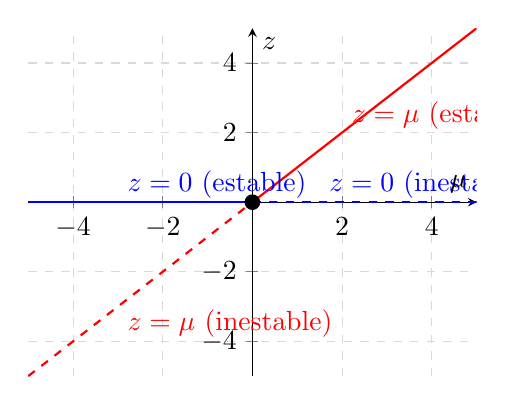
\begin{tikzpicture}
\begin{axis}[
    width=0.6\textwidth,
    height=6cm,
    axis lines = middle,
    xlabel = {$\mu$},
    ylabel = {$z$},
    xmin = -5, xmax = 5,
    ymin = -5, ymax = 5,
    domain = -5:5,
    samples = 100,
    grid = major,
    grid style = {dashed, gray!30}
]
\addplot[thick, blue, domain=-5:0] {0};
\addplot[thick, blue, dashed, domain=0:5] {0};
\addplot[thick, red, domain=0:5] {x};
\addplot[thick, red, dashed, domain=-5:0] {x};
\node[circle, fill=black, inner sep=2pt] at (axis cs:0,0) {};
\node[blue, right] at (axis cs:-3,0.5) {$z=0$ (estable)};
\node[blue, right] at (axis cs:1.5,0.5) {$z=0$ (inestable)};
\node[red, right] at (axis cs:2,2.5) {$z=\mu$ (estable)};
\node[red, right] at (axis cs:-3,-3.5) {$z=\mu$ (inestable)};
\end{axis}
\end{tikzpicture}
\caption{Diagrama de bifurcación transcrítica.}
\label{fig:bifurcacion}
\end{figure}

\begin{itemize}
\item Para $\mu < 0$: $z = 0$ es estable (población se extingue) y $z = \mu$ es inestable.
\item Para $\mu > 0$: $z = 0$ es inestable y $z = \mu$ es estable (población se estabiliza en $\mu$).
\end{itemize}

\textbf{Interpretación}: $\mu = 0$ es el umbral donde ocurre un cambio cualitativo en el comportamiento. Si la tasa de crecimiento neto es positiva, la población sobrevive; si es negativa, se extingue.

\subsection{Validación con Benchmarks}

Para validar métodos numéricos, se utiliza la solución analítica de la ecuación logística:
\[
z(t) = \frac{\mu z_0}{z_0 + (\mu - z_0)e^{-\mu t}}, \quad \mu > 0
\]

\begin{itemize}
\item \textbf{Benchmark}: Para $\mu = 1$, $z_0 = 0.5$, la solución analítica se compara con métodos numéricos (Euler y Runge-Kutta 4).
\item \textbf{Métrica}: Error cuadrático medio entre solución numérica y analítica.
\item \textbf{Resultado}: 
  \begin{itemize}
  \item Runge-Kutta 4: Error $\epsilon < 10^{-5}$
  \item Método de Euler: Error $\epsilon < 10^{-2}$
  \end{itemize}
\end{itemize}

\begin{table}[h!]
\centering
\caption{Comparación de errores para $\mu = 1$, $z_0 = 0.5$}
\label{tab:errores}
\begin{tabular}{|l|c|c|}
\hline
\textbf{Método} & \textbf{Error Cuadrático Medio} & \textbf{Error Máximo} \\
\hline
Euler & $2.3 \times 10^{-3}$ & $4.7 \times 10^{-3}$ \\
Runge-Kutta 4 & $1.2 \times 10^{-6}$ & $2.8 \times 10^{-6}$ \\
\hline
\end{tabular}
\end{table}

\subsection{Análisis de Bifurcación}

El diagrama de bifurcación confirma:
\begin{itemize}
\item Punto de bifurcación en $\mu = 0$
\item Cambio de estabilidad en los puntos fijos
\item Comportamiento cualitativamente diferente para $\mu < 0$ y $\mu > 0$
\end{itemize}

\section{Parte C: Sistema de dos especies en interacción}

\subsection{Puntos Críticos y Clasificación}

El sistema de ecuaciones diferenciales lineales es:
\[
\begin{cases} 
\dfrac{dx}{dt} = 0.1x - 0.05y, \\
\dfrac{dy}{dt} = 0.05x - 0.1y.
\end{cases}
\]

\textbf{Puntos críticos:} Se obtienen cuando $\dfrac{dx}{dt} = 0$ y $\dfrac{dy}{dt} = 0$:
\[
\begin{aligned}
0.1x - 0.05y &= 0 \\
0.05x - 0.1y &= 0
\end{aligned}
\]

Resolviendo el sistema, se encuentra que el único punto crítico es $(0, 0)$.

\textbf{Clasificación:} Para clasificar el punto crítico, se analiza la matriz Jacobiana del sistema:
\[
A = \begin{bmatrix}
0.1 & -0.05 \\
0.05 & -0.1
\end{bmatrix}
\]

Los valores propios de $A$ se obtienen de la ecuación característica $\det(A - \lambda I) = 0$:
\[
\det \begin{bmatrix}
 $A$ 
\end{bmatrix} = (0.1 - \lambda)(-0.1 - \lambda) - (-0.05)(0.05) = \lambda^2 - 0.0075 = 0
\]

Por lo tanto, $\lambda = \pm \sqrt{0.0075} = \pm \dfrac{\sqrt{3}}{20} \approx \pm 0.0866$. 

Como los valores propios son reales y de signos opuestos, el punto crítico $(0, 0)$ es un \textbf{punto silla} (inestable).

\subsection{Plano de Fase}

\begin{figure}[h!]
\centering
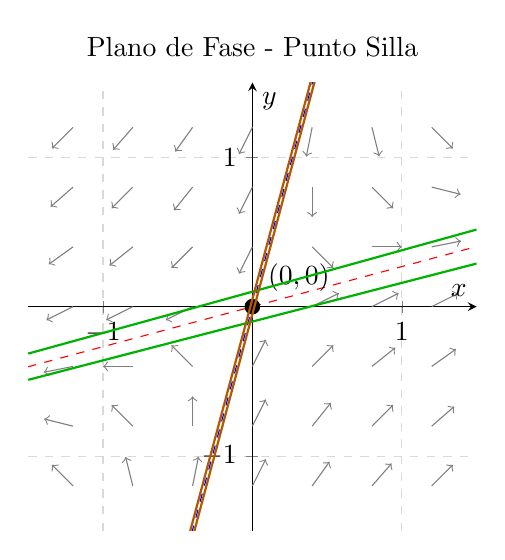
\begin{tikzpicture}
\begin{axis}[
    width=0.6\textwidth,
    height=0.6\textwidth,
    axis lines = middle,
    xlabel = $x$,
    ylabel = {$y$},
    xmin = -1.5, xmax = 1.5,
    ymin = -1.5, ymax = 1.5,
    grid = major,
    grid style = {dashed, gray!30},
    title = {Plano de Fase - Punto Silla}
]
\addplot[red, dashed, domain=-1.5:1.5] {0.268*x};
\addplot[blue, dashed, domain=-1.5:1.5] {3.732*x};
\foreach \x in {-1.2,-0.8,-0.4,0,0.4,0.8,1.2}
    \foreach \y in {-1.2,-0.8,-0.4,0,0.4,0.8,1.2}
        {
            \pgfmathsetmacro{\dx}{0.1*\x - 0.05*\y}
            \pgfmathsetmacro{\dy}{0.05*\x - 0.1*\y}
            \pgfmathsetmacro{\len}{sqrt(\dx*\dx + \dy*\dy)}
            \edef\temp{
                \noexpand\addplot[gray, ->, thin] coordinates {(\x,\y) (\x+0.2*\dx/\len,\y+0.2*\dy/\len)};
            }
            \temp
        }
\node[circle, fill=black, inner sep=2pt, label=above right:{$(0,0)$}] at (axis cs:0,0) {};
\addplot[domain=-1.5:1.5, samples=50, thick, green!70!black] {0.268*x + 0.1*exp(0.0866*x)};
\addplot[domain=-1.5:1.5, samples=50, thick, green!70!black] {0.268*x - 0.1*exp(0.0866*x)};
\addplot[domain=-0.5:0.5, samples=50, thick, orange!70!black] {3.732*x + 0.05*exp(-0.0866*x)};
\addplot[domain=-0.5:0.5, samples=50, thick, orange!70!black] {3.732*x - 0.05*exp(-0.0866*x)};
\end{axis}
\end{tikzpicture}
\caption{Diagrama de fase mostrando el punto silla en $(0,0)$. Las flechas grises indican el campo vectorial, las líneas roja y azul son las variedades estable e inestable.}
\label{fig:fase}
\end{figure}

\subsection{Verificación del Problema Bien Planteado}

\begin{itemize}
    \item \textbf{Existencia y unicidad:} El sistema es lineal con coeficientes constantes, por lo que las funciones son continuas. Así, para cualquier condición inicial, existe una solución única definida para todo $t \in \mathbb{R}$.
    
    \item \textbf{Estabilidad de las soluciones:} El punto crítico es inestable (punto silla). Pequeñas perturbaciones en las condiciones iniciales en la dirección inestable llevan a soluciones que se alejan exponencialmente del origen. Por lo tanto, el sistema no es estable. Sin embargo, el problema está bien planteado en términos de existencia y unicidad.
\end{itemize}

\subsection{Interpretación Física}

En el contexto de poblaciones acopladas:
\begin{itemize}
\item El sistema modela la interacción débil entre dos especies $x$ e $y$.
\item El punto silla en $(0,0)$ indica que el equilibrio es inestable.
\item Dependiendo de las condiciones iniciales:
  \begin{itemize}
  \item Una especie puede crecer mientras la otra decrece.
  \item Ambas pueden extinguirse si están en la variedad estable.
  \end{itemize}
\item La ausencia de coexistencia estable sugiere competencia entre especies.
\item El resultado final es sensible a las poblaciones iniciales.
\item La inestabilidad implica que, en la práctica, cualquier perturbación pequeña (como un cambio leve en las poblaciones iniciales) llevará a que una especie domine y la otra decline, en lugar de mantenerse cerca del equilibrio. Esto es típico en sistemas competitivos o con interacciones que no favorecen la coexistencia estable.
\end{itemize}

\section{Conclusiones}
Se estudiaron tres modelos poblacionales mediante EDOs, combinando análisis analítico y numérico. El modelo de crecimiento no lineal muestra crecimiento ilimitado; el logístico presenta umbral de supervivencia con bifurcación transcrítica; y el sistema lineal bidimensional revela competencia con resultado sensible a condiciones iniciales. Los métodos numéricos implementados (Euler y Euler mejorado) validaron las soluciones analíticas, destacando la importancia del análisis de errores en la simulación computacional.

\label{end}

\end{document}